\begin{figure*}[!t]
\small
  \centering
  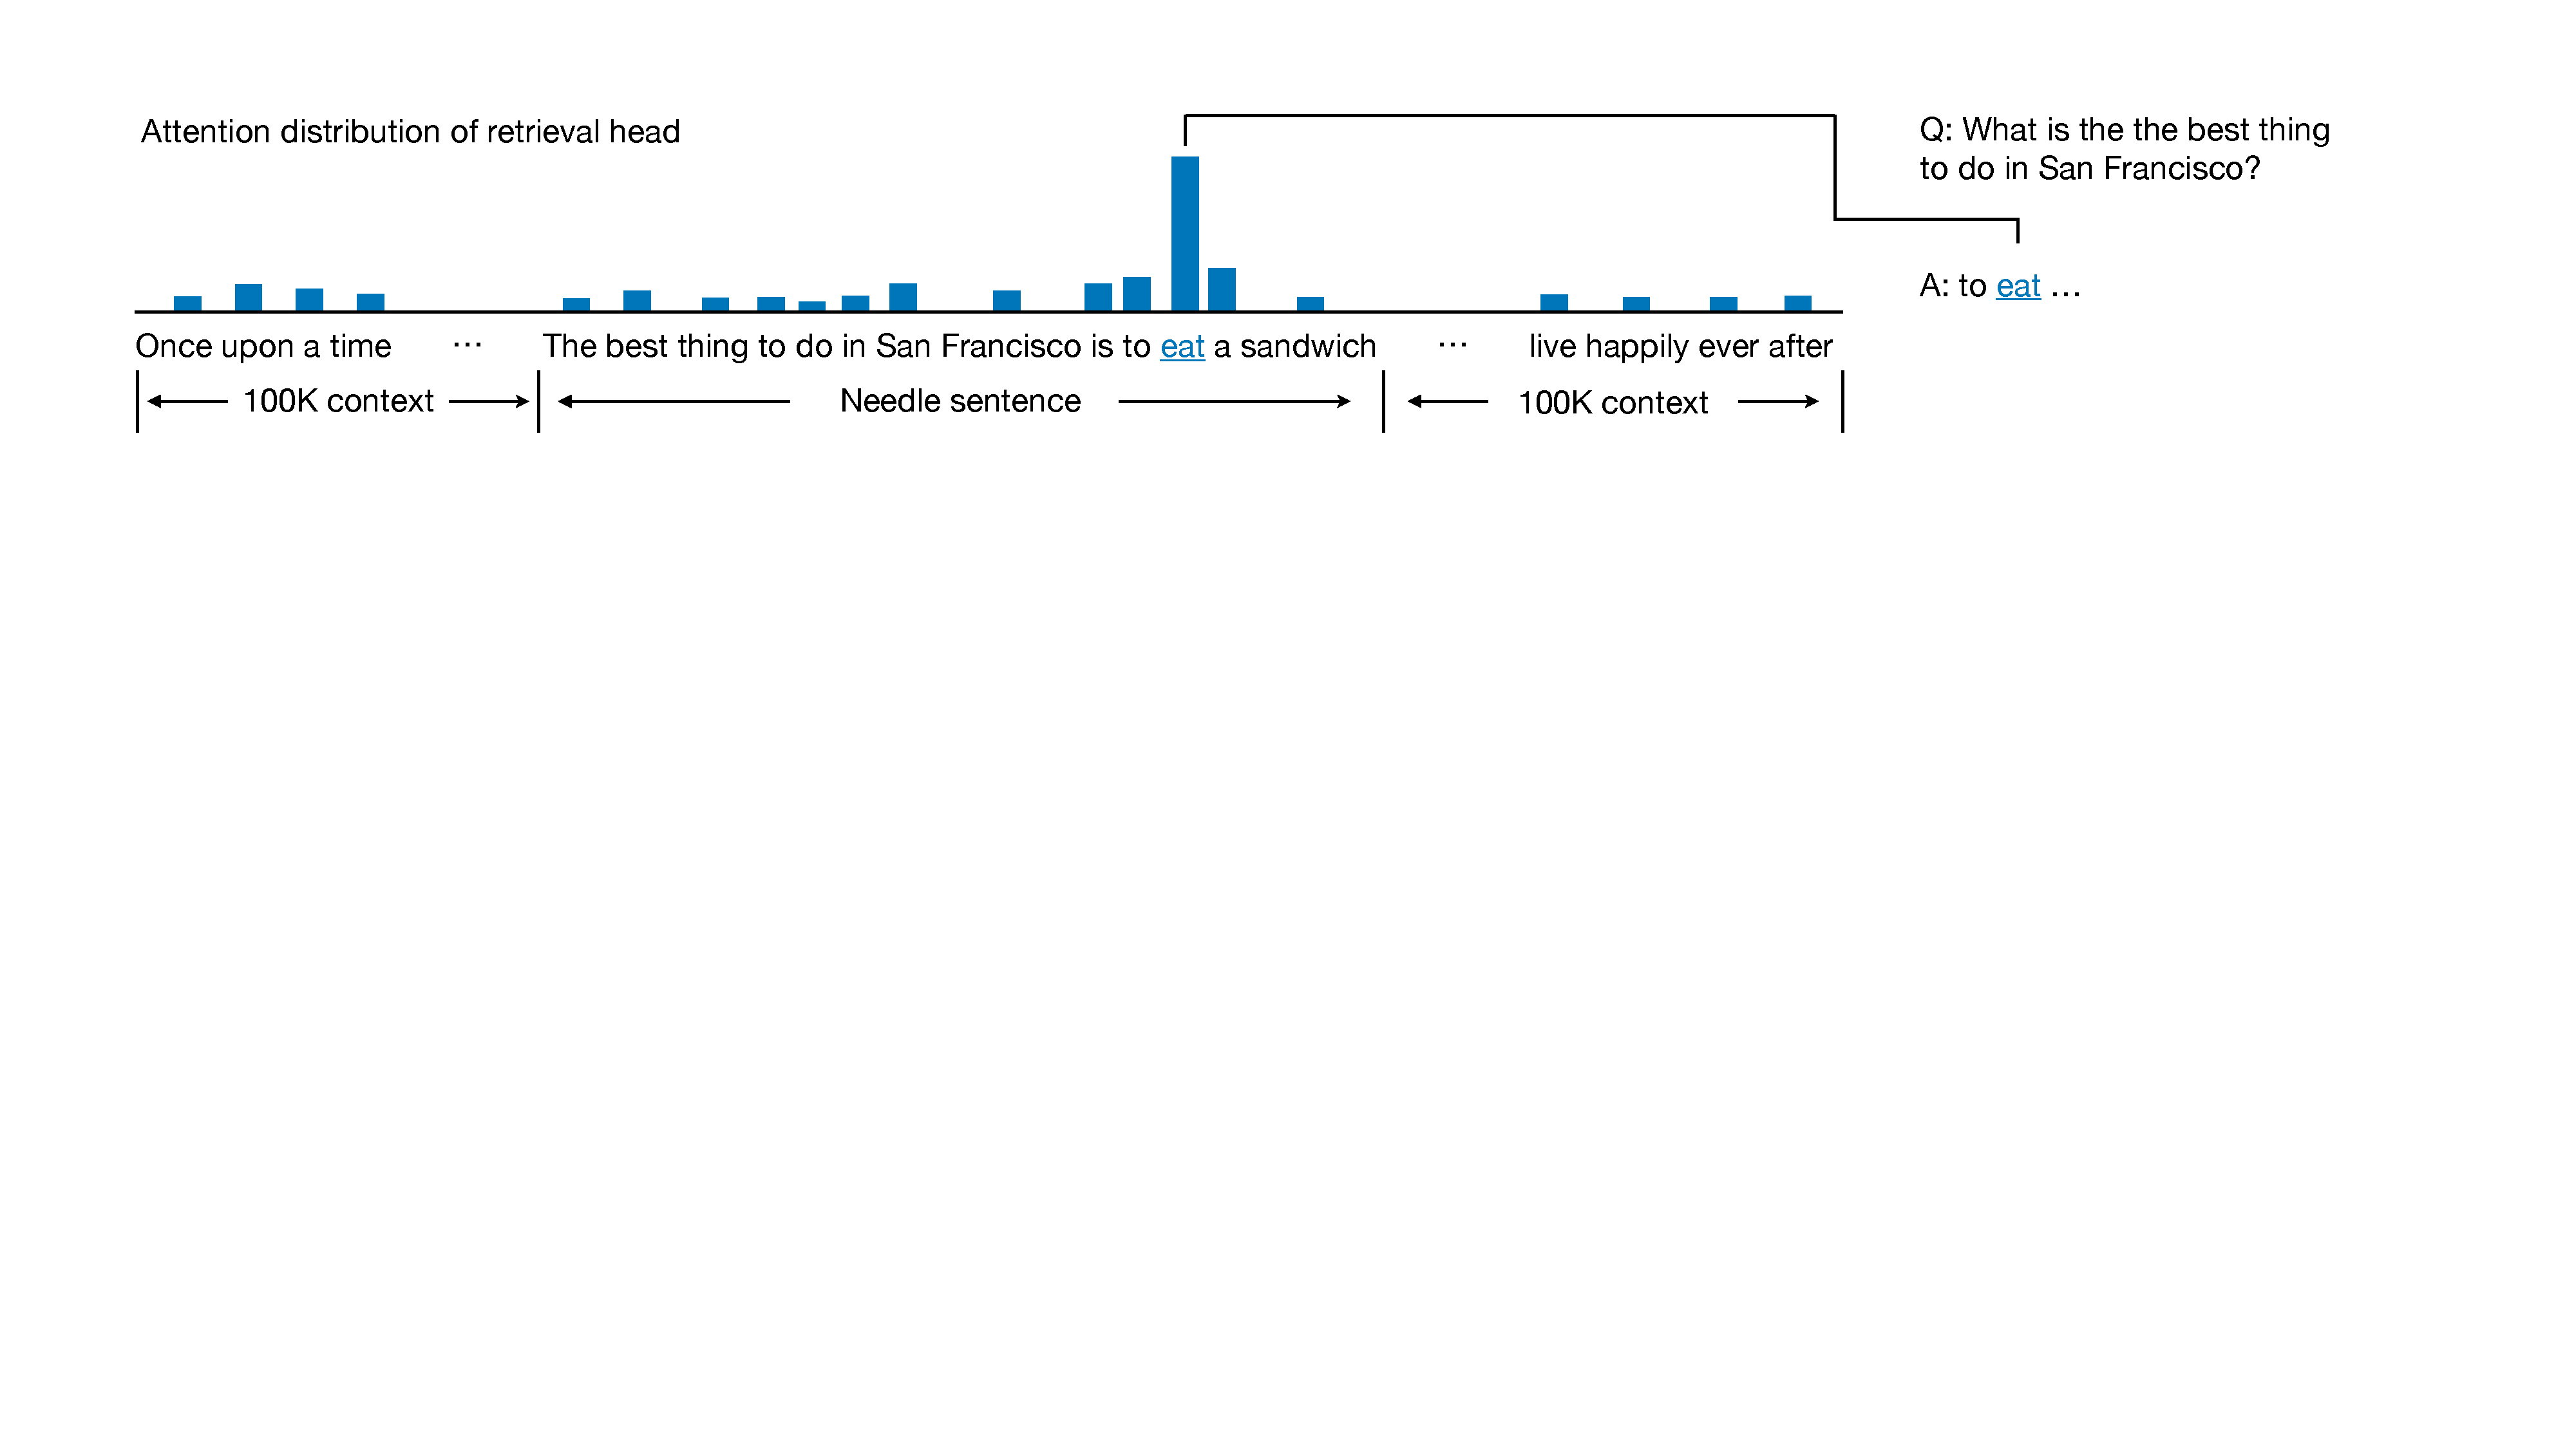
\includegraphics[width=\linewidth]{figures/retrieval_attention_dist.pdf}
  \caption{An attention head that performs a copy-paste operation if the token that the head attend to is the same the token being generated. 
  The retrieval score of a head is defined as the frequency of this head's copy-paste behavior when answering quesions that asks for raw information from the input. 
  }
  \label{fig:retrieval_attention_dist}
\end{figure*}

\begin{table*}[t!]
    \centering
    % \renewcommand{\arraystretch}{1}
    % \setlength{\tabcolsep}{5.5pt}
    \caption{\label{tab:all_models} We consider a wide range of language model families and show that the basic properties of retrieval heads are universal and consistent across all language models we study. }
    \begin{tabular}{@{}l|l|l@{}}
    \toprule
     \bf  Base Model& \bf Variant & \bf Variation Type\\
         \midrule

     Llama-2-7B& Llama-2-7B-80K & Length Extension via Continue Pretrain\\
     &Llama-2-13B-64K & Model Scaling and Length Extension\\
          \midrule

     Mistral-7B-v0.2 & Mistral-7B-Instruct-v0.2 & SFT and RLHF\\
     & Mixtral-8x7B-v0.1 & Sparse Upcycling to Mixture of Experts\\
     \midrule
     Yi-6B      & Yi-6B-200K & Length Extension via Continue Pretrain\\
                & Yi-34B-200K & Model Scaling and Length Extension\\
     \midrule
     Qwen1.5-14B & Qwen1.5-14B-Chat& SFT and RLHF\\
     \toprule
    \end{tabular}
\end{table*}


To detect which head is implementing the retrieval algorithm, we introduct a \textit{retrieval score} to measures the frequency of a head's copy-paste behavior during autoregressive decoding. 
An attention head with high retrieval score suggests that statistically across various contexts, this head is frequently copying the input tokens from the input to the output. 


\textbf{Needle-in-a-Haystack}\quad\quad Our retrieval head detection algorithm roots from the needle-in-a-Haystack test, which asks the model to copy-paste the input tokens to the output.
Given a question $\vq$ and its corresponding answer $\vk$ (the needle),  we insert $\vk$ in a given context  $\vx$  (the haystack) at a random position index range $\vi_q$.
The language model is then tasked with answering $\vq$ based on the haystack with the inserted needle.
We set $\vq$ and $\vk$ unique and irrelevant with the given long context,
ensuring that if an answer is correctly generated, it is indeed copied from the context, not from the model's internal knowledge.

\textbf{Retrieval Score for Attention Heads}\quad\quad 
We define the retrieval score as the frequency of a head's copy-paste operations. 
Specifically, 
during auto-regressive decoding (we use greedy decoding by default), 
denote the current token being generated as $w$ and
the attention scores of a head as $\boldsymbol{a} \in \mathcal{R}^{|\vx|}$.
As demonstrated in Fig.~\ref{fig:retrieval_attention_dist}, we say an attention head $h$ copies and pastes a token from the needle to the output sentence if it follows two criteria: 
(1) $w \in \vk$, i.e., $w$ is a token within the needle sentence. (2)
$\vx_j= w, j = \arg\max(\boldsymbol{a}), j \in \vi_q$, i.e., the input token that receives the most attention probability mass by this head is a token within the needle and is the same token as the currently generated token. 
Let $\vg_h$ be the set containing all tokens copy and pasted by a given head $h$, we define:
%
\begin{equation}
    \text{Retrieval score for head}\;\; h = \frac{|\vg_h \cap \vk |}{|\vk|}, 
\end{equation}
%
Intuitively, retrieval score  represents a token-level recall rate of the most attended tokens by an attention head.
For example, when retrieving a needle of 10 tokens, a retrieval score of 0.9 indicates that the attention head has copies and pasted 9 tokens in the 10-token target answer.

\textbf{Retrieval Head Detection Algorithm}\quad\quad
We calculate the retrieval score for all attention heads under a diverse set of input contexts. 
For each language model we consider, we compile three sets of Needle-in-a-Haystack samples, each consisting of a unique tuple $(\vq, \vk, \vx)$.
For each sample, we make sure $(\vq, \vk)$ is semantically irrelevant with $\vx$ and that $\vq$ cannot be answered using the model's existing knowledge by manually inspecting the model output. 
Then for each $(\vq, \vk, \vx)$ sample, we perform  Needle-in-a-Haystack on 20 different length values uniformly sampled from 1K-50K, where in each length, $\vq$ is inserted in 10 different depth uniformly ranging from the start to the end of $\vx$.
We note that this scale of tests gives stable outputs as the average retrieval score converges after just a few samples. 
In total, each language model is subjected to approximately 600 instances of retrieval testing. 
We calculate the retrieval score for each attention head in each test and use the average of these scores as the head's final retrieval score.
The attention heads with relatively larger retrieve score  can be considered as retrieval head.
In our case (Fig.~\ref{fig:score_range}), we set the threshold as 0.1, meaning that as long as the head performs copy-paste in 10\% of the times, we consider it a retrieval head. 
